\section*{WRITING TASK 1}
You should spend about 20 minutes on this task.

\begin{quote}\large The pie charts show how household energy use was distributed among four purposes in a fictional country in 2000 and 2025.
\end{quote}
Describe the main features of the information, select relevant details, and make comparisons where appropriate.

\begin{center}
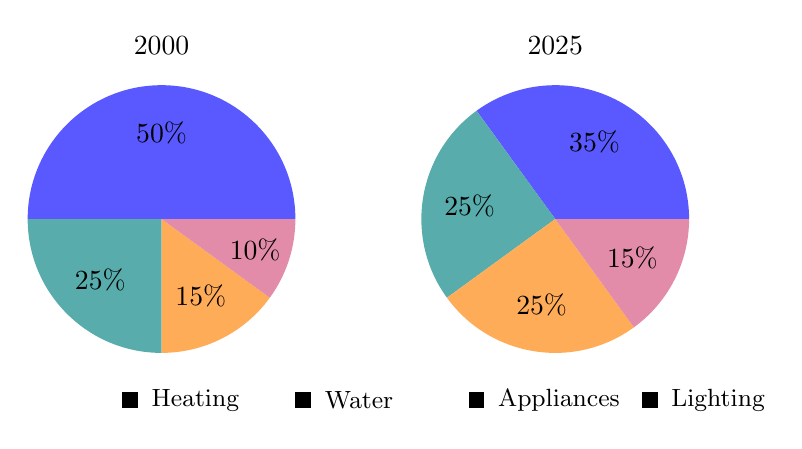
\begin{tikzpicture}
\begin{scope}[shift={(0,0)}]
\fill[blue!65] (0,0)--(0:1.7) arc (0:180:1.7)--cycle;
\fill[teal!65] (0,0)--(180:1.7) arc (180:270:1.7)--cycle;
\fill[orange!65] (0,0)--(270:1.7) arc (270:324:1.7)--cycle;
\fill[purple!45] (0,0)--(324:1.7) arc (324:360:1.7)--cycle;
\node at (0,2.2){2000};\node at (90:1.1){50\%};\node at (225:1.1){25\%};\node at (297:1.1){15\%};\node at (342:1.25){10\%};
\end{scope}
\begin{scope}[shift={(5,0)}]
\fill[blue!65] (0,0)--(0:1.7) arc (0:126:1.7)--cycle;
\fill[teal!65] (0,0)--(126:1.7) arc (126:216:1.7)--cycle;
\fill[orange!65] (0,0)--(216:1.7) arc (216:306:1.7)--cycle;
\fill[purple!45] (0,0)--(306:1.7) arc (306:360:1.7)--cycle;
\node at (0,2.2){2025};\node at (63:1.1){35\%};\node at (171:1.1){25\%};\node at (261:1.1){25\%};\node at (333:1.1){15\%};
\end{scope}
\foreach \x/\color/\name in {-0.5/blue/Heating,1.7/teal/Water,3.9/orange/Appliances,6.1/purple/Lighting}{\fill[\color!65] (\x,-2.4) rectangle +(0.2,0.2);\node[anchor=west,font=\small] at (\x+0.25,-2.3){\name};}
\end{tikzpicture}
\end{center}
Write at least 150 words.
\par\bigskip
{\footnotesize\color{gray} Original practice material; fictional settings and data. Not an official IELTS examination paper.}
